\documentclass[a4paper]{article}

\usepackage{graphicx}
\usepackage[tuenc]{fontspec}
\usepackage{xcolor}

\usepackage[hidelinks]{hyperref}
\usepackage{csquotes}
\usepackage[english]{babel}
\usepackage[
    backend=biber,
    sorting=none
]{biblatex}

\setmainfont{CMU Serif}
\setlength{\parskip}{\baselineskip}

% Bibliography
\addbibresource{lliurable.bib}

    
\begin{document}

\begin{titlepage}
    \centering
	\vspace{1.5cm}
	{\huge \textbf{\textsc{Unlock the potential of medical imaging data using deep learning}} \par}
	\vspace{2cm}
	{\Large \textit{Joan Marcè i Igual}\par}
	\vfill
    Director: Dr.Benjamin \textsc{Haibe-Kains}
    
    \vfill

    
\includegraphics[width=0.2\textwidth]{images/logo_upc}\par\vspace{1cm}
	\vfill
    
    % Bottom of the page
    {\LARGE Universitat Politècnica de Catalunya \par}
    {\LARGE 2018 \par}
\end{titlepage}

\tableofcontents

\section{Context}

\subsection{Problem formulation}

Nowadays one of the most extensive uses of computing is artificial intelligence. This is being
used from based on our preferences help us to select what products we can buy to properly detect
and focus faces when taking a picture. The main advantage of this field is that it reduces the
amount of human intervention and usually it performs better.

Inside AI one of the domains that has greatly increased during the last years is 
\emph{Machine Learning}. The main advantage is that it can solely learn from examples without 
explicit teaching, and thus reducing the human interaction during the learning process. One of the 
most used types is \emph{deep neural networks} and these have demonstrated impressive performance 
against task like the classification of digit from the MNIST data set.
~\cites{MNIST}{empirical-evaluation-deep-architectures}

Regarding the medical field, recent deep learning algorithms, specially convolutional networks. 
Traditionally medical predictions have been based on a few clinical parameters with poor accuracy.
However, other data types are available to improve such predictions. In this context, medical
images generated from MRI, PET or CT scans are vastly underused due to the inability of radiologists
to quantitatively analyze these complex data. 

Different methods have appeared to analyze these images for tasks such as
image classification, object detection, segmentation and registration among other tasks. This
approach started in the late 1990s and has slowly shifted from systems that are completely designed
by humans to systems that are trained by computers using example data. 
~\cite{survey-deep-learning}

To use all this data Survival Prediction models have been created. This type of models are
used to understand the relations between patients and effectiveness of various treatment options. 
The survival and hazard functions are the two fundamental functions in survival analysis. The
survival function \( S(t) = \Pr(T > t) \), is the probability that an individual has
\emph{survived} beyond time \( t \). The hazard function is a measure of risk at time \( t \).
The hazard function \( \lambda(t) \) is defined as:
~\cite{DeepSurv}
\[
    \lambda(t) = \lim_{\delta \rightarrow 0}
    \frac{\Pr(t \le T < t + \delta | T \ge t)}{\delta}
\]


Also, to compare if an algorithm is performing better than another one we usually use the ROC curve
example which compares the \emph{False Positive Rate} against the \emph{True Positive Rate},
see \autoref{fig:ROC-curve}. The Cox Proportional Hazards (CPH) model provides a starting point for a 
survival model and the future models will be compared against this one.
~\cites{ROC-precision-recall}{Cox}

\begin{figure}
    \centering
    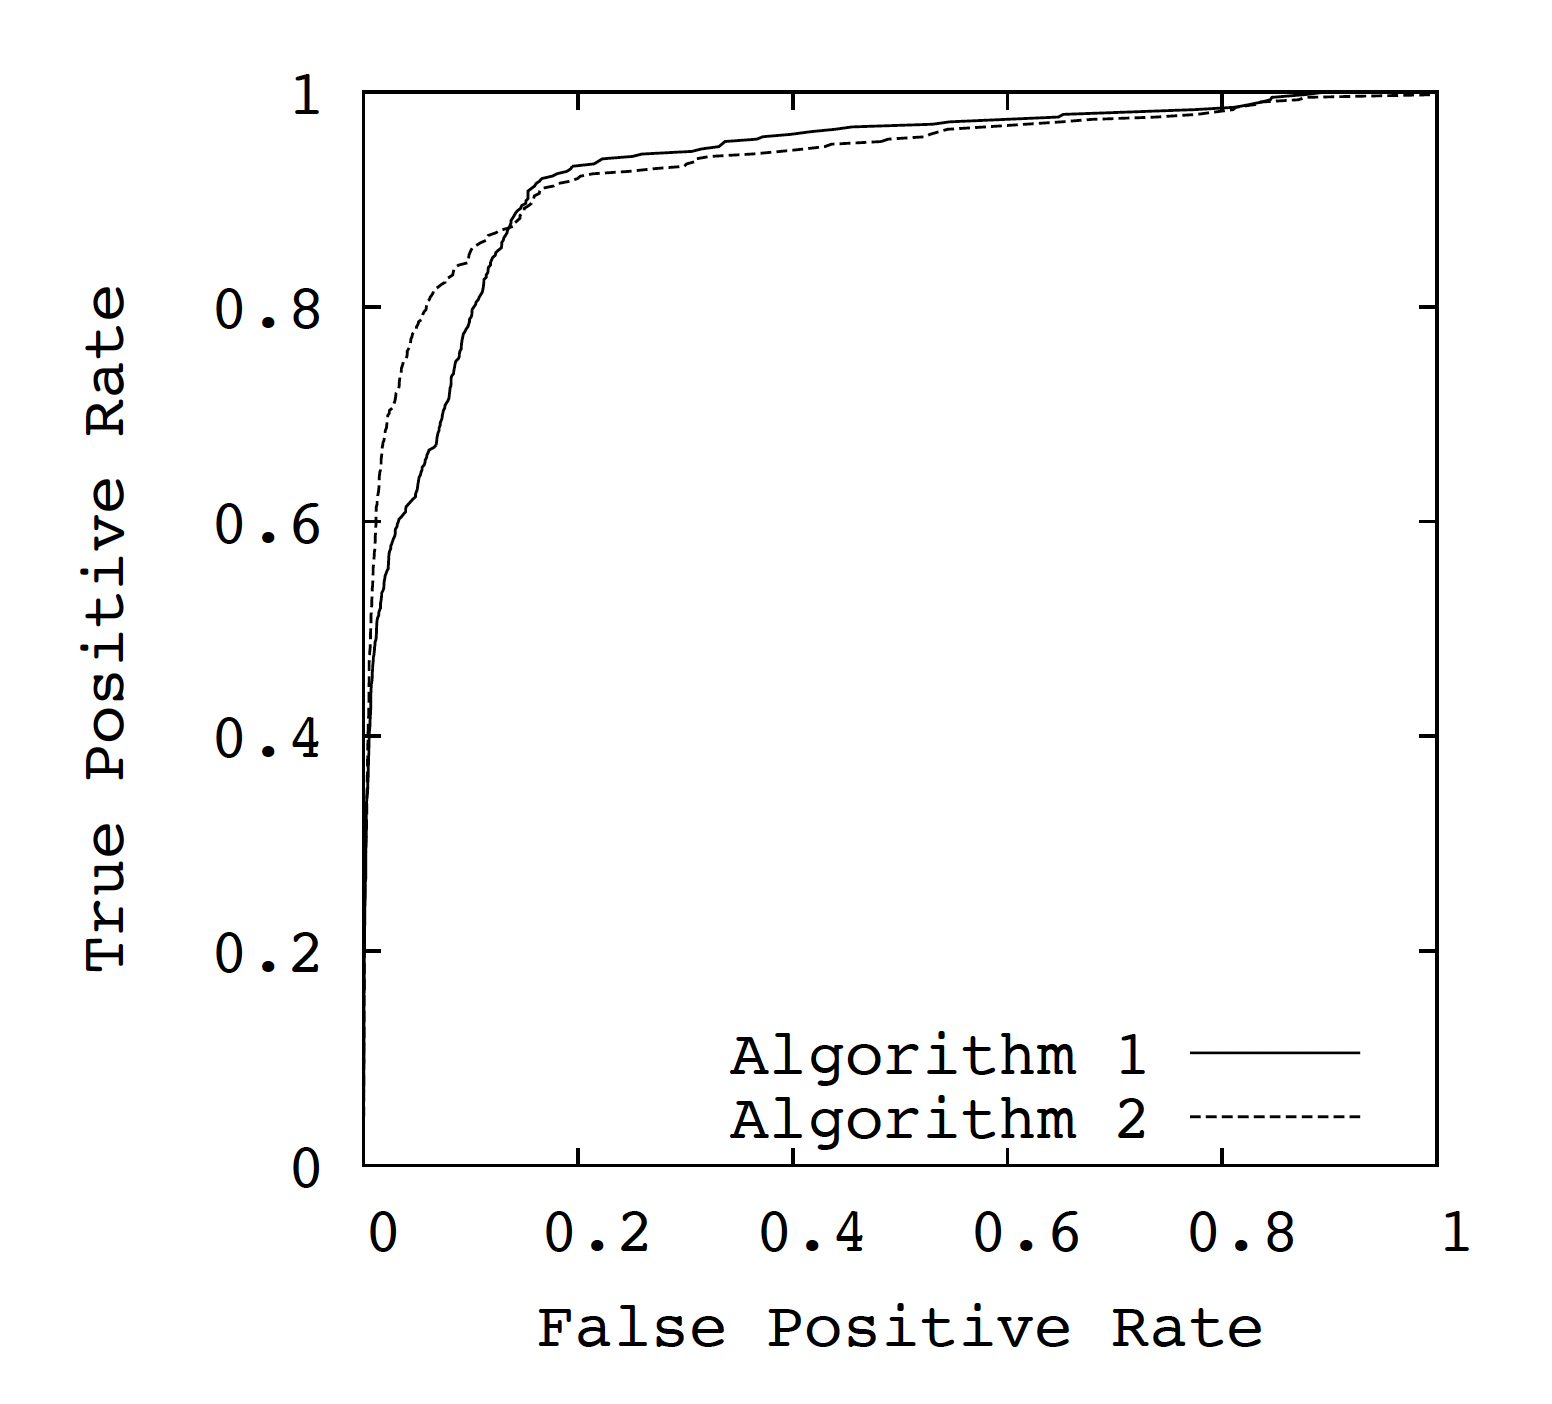
\includegraphics[width=.5\linewidth]{images/roc_curve}
    \caption{ROC Curve example\label{fig:ROC-curve}}
\end{figure}

The goal of this project is to apply the current known methods to create a model for prediction
of survival in head and neck cancer patients. This model will be created with 

With help from professor Benjamin Haibe-Kains which has helped in the development of 
\emph{Radiomics}, a new field to better characterize tumors and predict survival outcome and 
Dr.~Fei-Fei Liu, head of the Radiation Medicine Program at the Princess Margaret Cancer Centre. 
Both have access to a unique set of \~500 scans of head-and-neck cancer patients with associated 
survival data. 

% TODO: I stopped here!
Moreover, Benjamin Haibe-Kains lab has been involved in the development of radiomics, a new field 
relying on pre-defined, hand-engineered features computed from medical images to better characterize 
tumors and predict survival outcome. Although promising, radiomics suffers from two several 
limitations: (i) the number of features is limited (~1200) and (ii) it is a slow process as it 
requires a radiologist to manually contour the tumor. Deep learning has the potential to
address both issues by automatically extracting more information from the images.
~\cite{deep-learning-radiomics-gbm}

I am happy to invite you in my lab from the 1st of February to the 31st of July through CFIS (Interdisciplinary
Higher Education Centre) to work on the project entitled “Unlock the potential of medical imaging data using
deep learning”. In this era of BIG data science, recent deep learning algorithms are pushing the boundaries of
precision medicine in cancer with the aim to predict the best treatment strategy for each patient. Traditionally
such predictions are based on a few clinical parameters with poor accuracy. However, other data types are
available to improve such predictions. In this context, medical images generated from MRI, PET or CT scans
are vastly underused due to the inability of radiologists to quantitatively analyze these complex data. My lab
has been involved in the development of radiomics, a new field relying on pre-defined, hand-engineered
features computed from medical images to better characterize tumors and predict survival outcome. Although
promising, radiomics suffers from two severa limitations: (i) the number of features is limited (~1200) and (ii) it
is a slow process as it requires a radiologist to manually contour the tumor. Deep learning has the potential to
address both issues by automatically extracting more information from the images.
Through our collaboration with Dr. Fei-Fei Liu, head of the Radiation Medicine Program at the Princess
Margaret Cancer Centre, my lab has access to a unique set of ~500 scans of head-and-neck cancer patients
with associated survival data. The goal of this project is to develop a new deep learning framework to analyze
this private dataset in combination with public databases to improve the prediction rate of patients’ survival
compared to models built on traditional radiomic features. I expect you to explore the use of dropout and image
augmentation techniques to improve the fitting of neural networks from medical images. You will work in close
collaboration with radiologists and experts in machine learning in my lab and will participate to the redaction of
the manuscript describing the analysis results.


The main objective of this project is to try to apply the current known methods, like DeepSurv, 
for survival prediction and create a 

\subsection{Stakeholders}

\subsubsection{Developer}
\subsubsection{Physicians and Hospitals}
\subsubsection{Patients}

\section{State-of-the-art}

\section{Scope}

\pagebreak
\printbibliography{}

\end{document}